\documentclass[a4paper,11pt,final]{article}
\usepackage[top=2cm,left=2cm,right=2cm,bottom=2cm]{geometry}% margins
\usepackage{graphicx}
\usepackage{helvet}
\renewcommand{\familydefault}{\sfdefault}
\pagestyle{empty}					% no pagenumbering
\setlength{\parindent}{0pt}			% no paragraph indentation
\usepackage{flowfram}										% column 										% figures
\usepackage{url}											% URLs
\usepackage[usenames,dvipsnames]{xcolor}					% color
\usepackage{multicol}										% columns 
\usepackage{tikz}
\setlength{\multicolsep}{0pt}
\usepackage{paralist}										% compact lists
\usepackage{tikz}
\setlength{\vcolumnsep}{\baselineskip}
\setlength{\columnsep}{\vcolumnsep}


\newcommand{\CVSection}[1]
{\Large\textbf{#1}\par
	\SmallSep\normalsize\normalfont}

\newcommand{\CVItem}[1]
{\textbf{\color{Black} #1}}
\newcommand{\Sep}{\vspace{1.5em}}
\newcommand{\SmallSep}{\vspace{0.5em}}
\usepackage[hidelinks]{hyperref}

\begin{document}
	
	\begin{minipage}{0.8\textwidth}% adapt widths of minipages to your needs
	\Large \textbf{Bishwamittra Ghosh}\\
	\normalsize PhD Student,\\
	 Computer Science Department, School of Computing,\\
	 National University of Singapore.\\
	 Email: \url{bishwa@comp.nus.edu.sg}  \\
	 Website: \url{https://bishwamittra.github.io}
	\end{minipage}%
	\hfill%
	\begin{minipage}{0.2\textwidth}
		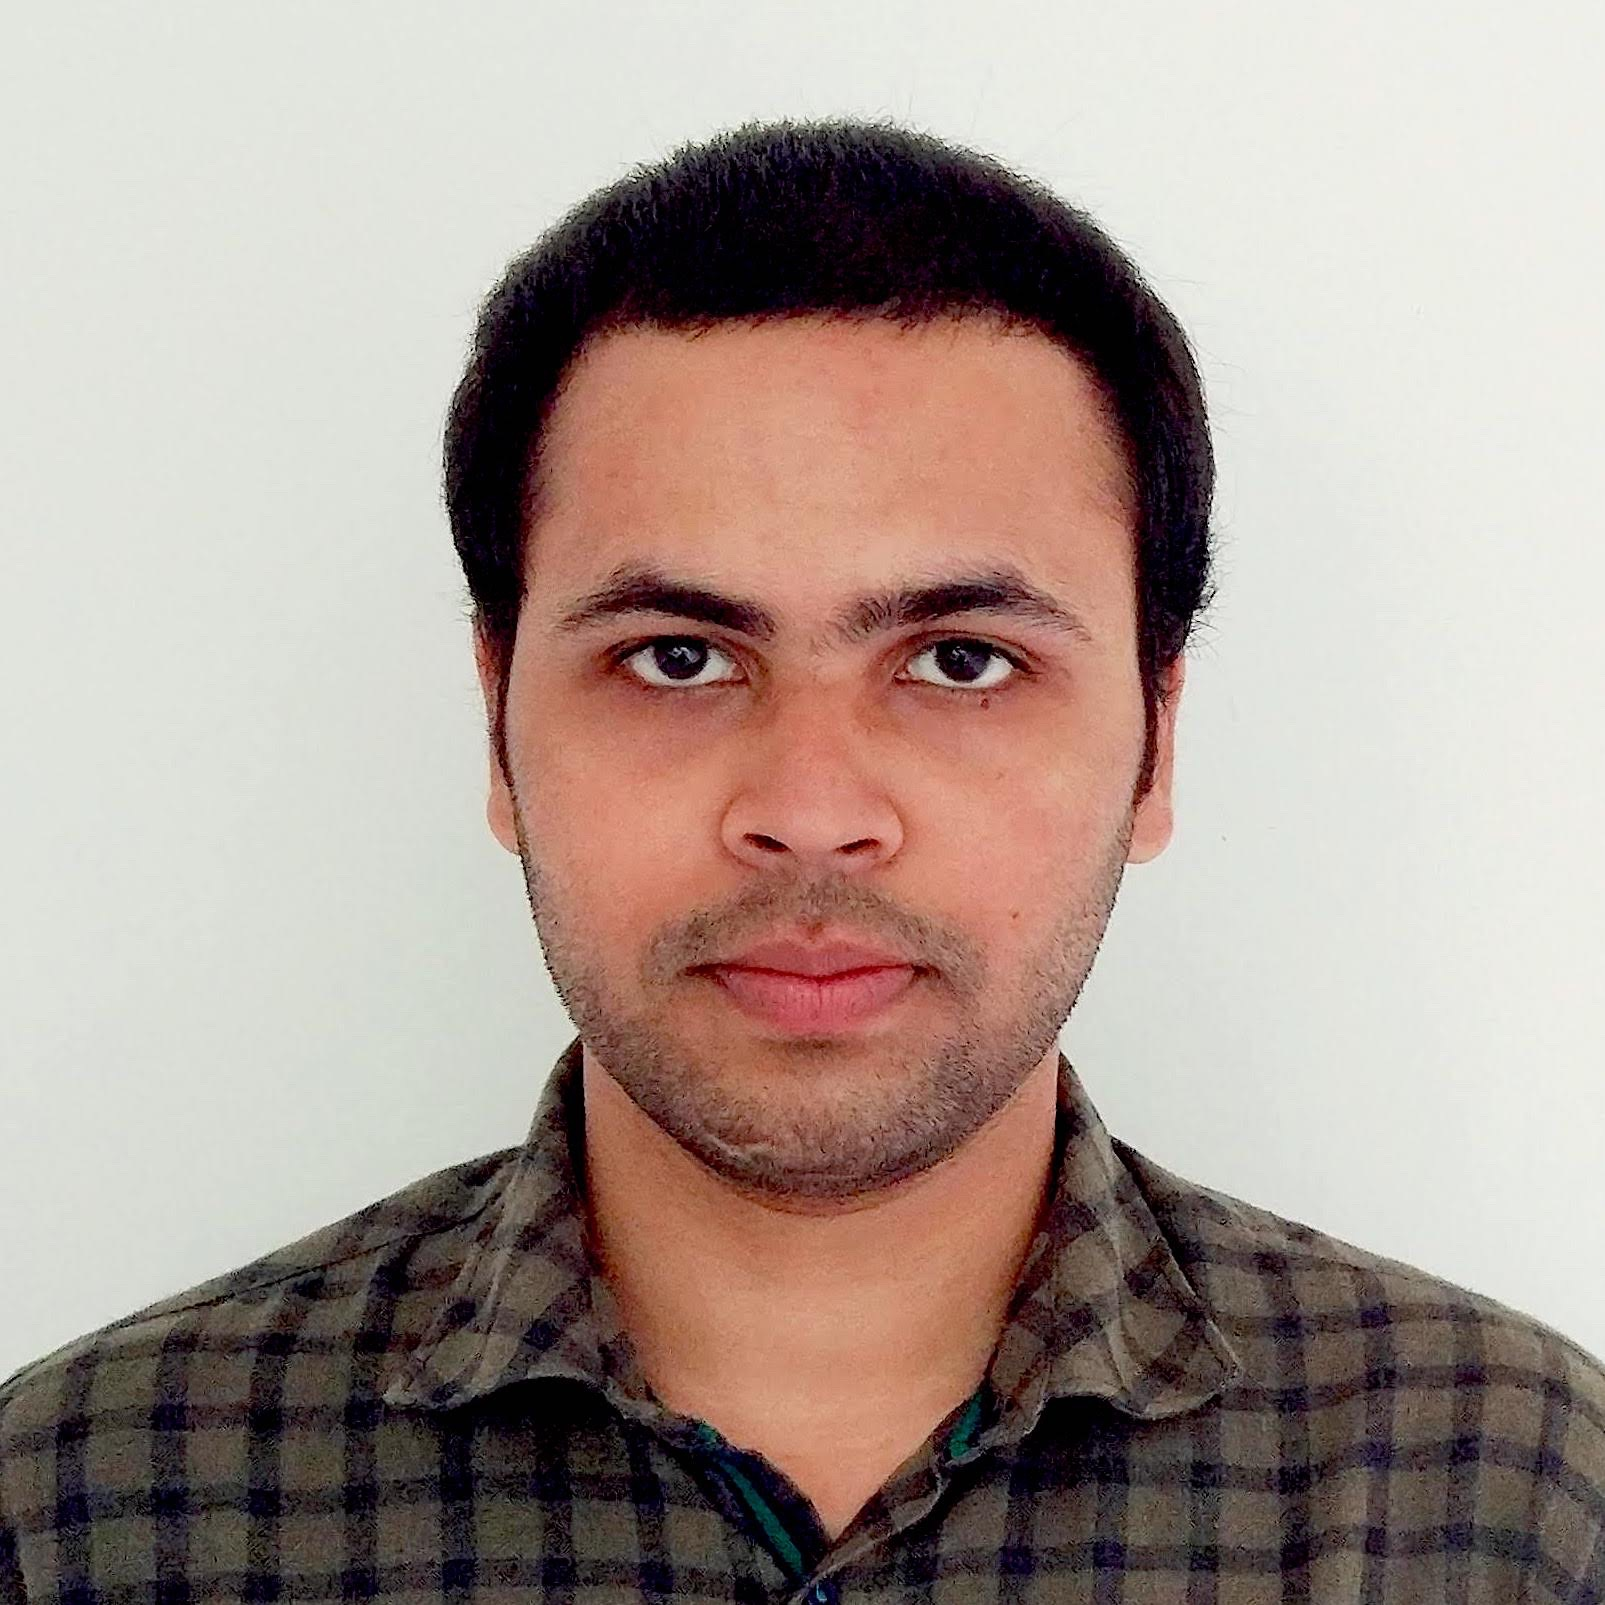
\includegraphics[width=\linewidth]{photo.jpg}
		
	\end{minipage}


\vspace{.5 cm}
\Large \centerline{ \textbf{Curriculum Vitae}}
\vspace{.5 cm}
\normalsize
\normalfont
\CVItem{Date of Birth:}  28  November,  1995 \\
\CVItem{Place of Birth:} Satkhira, Bangladesh\\
\CVItem{Citizenship:} Bangladesh\\

\CVSection{Education}
\CVItem{ 2018  - On going}\\
PhD, Computer Science Department, School of Computing, National University of Singapore.
\SmallSep

\CVItem{ 2013  -  2017 }\\
BSc, Department of CSE, BUET, Bangladesh
\SmallSep

\CVItem{ 2010  -  2012 }\\
HSC, Satkhira Govt. College, Satkhira, Bangladesh 
\SmallSep

\CVItem{ 2008  -  2010 }\\
HSC, Satkhira Govt. High School, Satkhira, Bangladesh


\Sep
\CVSection{Research Interest:}
\begin{itemize}
	\item Constraint Programming
	\item SAT solving
	\item Explainable AI
\end{itemize}


\Sep
\CVSection{Selected Publications}
\begin{itemize}
	\item \CVItem{Interpretable Classification Rules in Relaxed Logical Form}\\
	Bishwamittra Ghosh, Dmitry Malioutov, Kuldeep S. Meel.\\
	IJCAI 2019 workshop on XAI (Explainable Artificial Intelligence) and DSO (Data Science meets Optimization).
	\item \CVItem{IMLI: An Incremental Framework for MaxSAT-Based Learning of Interpretable \\ Classification Rules}\\
	Bishwamittra Ghosh, Kuldeep S. Meel.\\
	Proceedings of AAAI/ACM Conference on AI, Ethics, and Society (AIES), 2019.
	\item \CVItem{The Flexible Socio Spatial Group Queries}\\
	Bishwamittra Ghosh, Mohammed Eunus Ali, Farhana M. Choudhury,
	Sajid Hasan Apon, Timos Sellis, Jianxin Li.\\
	Proceedings of the VLDB Endowment (PVLDB), 2019.
\end{itemize}





\newpage
\CVSection{Awards}
\CVItem{NUS Research Scholarship}\\
National University of Singapore.\\


\CVItem{Academic Merit Scholarship }
\\Dean's award,\\
Bangladesh University of Engineering and Technology .\\

\CVItem{Math Olympiad}\\
Camper for IMO.
\\
National and regional winner in Higher secondary, secondary, and junior level.\\

\CVItem{Scholarship}\\
Board scholarship in HSC, SSC, junior, and primary.





\Sep
\CVSection{References}
\begin{itemize}
	\item \textbf{Kuldeep S. Meel}\\
	Assistant Professor,\\
	School of Computing, National University of Singapore
	\item \textbf{Dr. Mohammed Eunus Ali }\\
	Professor,\\
	Department of CSE, BUET
\end{itemize}	



	
\end{document}
